\chapter{Theoretical Background}
\label{ch:theory}

This chapter attends to the theoretical background for the technologies used in this thesis.

\section{Convolutional Neural Networks}

\section{Word Representations}

\subsection{Glove}

\subsection{FastText}

\subsection{Elmo}

\section{Google Transformer Architecture}
\subsection{Positional Encoding}
\subsection{Attention Mechanism}
\subsection{Pointwise Layer}

\subsection{Xavier Initialization}

\subsection{Adam}

\subsection{NOAM}

\section{Multi-Task Learning}

Rich Caruana first introduced \acrfull{mtl} in 1993. Conventional machine learning approaches break a problem down in smaller tasks and solve one task at a time (e.g., word-by-word \gls{pos}-tagging \cite{Toutanova2007}, word-by-word \gls{ner} \cite{Sang2003} or handwritten image classification \cite{LeCun;1990}). In each of these tasks a classification algorithm solves exactly one task (Assigning a 'part-of-speech' or entity type to a word, or the classification of handwritten digits). Caruana shows that combining multiple related tasks improves model performance \cite{Caruana1993}\cite{Caruana1997a}. 

In \gls{mtl}, multiple related tasks are learned in parallel and share a common representation. Generally speaking every machine learning model which optimizes multiple objectives for a single sample can be considered as Multitask Learning. This includes multi-label classification where one sample can have multiple labels as well as instances where different sample distributions or datasets are used for different tasks.

\gls{mtl} is similar to how humans learn. Generally, humans learn new tasks by applying knowledge from previous experiences and activities. For instance, it is easier to learn ice skating when someone previously learned inline skating. This is because all the underlying important aspects of the tasks are very similar.

When tasks are related this also holds true for machine learning. When learning these tasks in parallel model performance is improved compared to learning them individually since the additional knowledge that a related task carries, can be used to improve on the original task \cite{Caruana1997a}. 

There are four important aspects one can use to determine if \gls{mtl} can bring performance boosts for a specific objective:
\begin{enumerate}
	\item Multi Label Task: Multi Label classification task where one sample can have more than one label are almost always inherintly solved using \gls{mtl} if labels are predicted by one model. Multiple authors show that adding tasks always improves performance compared to a separate model for each task as an alternative \cite{Ramsundar2015}. %TODO: More citations
	\item Shared low-level features: \gls{mtl} only makes sense if the tasks share low level features. For instance, image classification and \gls{nlp} do not share common features. In this case the model would not benefit from \gls{mtl} because one task can not help to improve the other task. Therefore, it is important to choose tasks that are related to each other \cite{Zhang2017a}. In most cases \gls{mtl} will work with \gls{nlp} tasks because they usually share at least some kind of sentence or word embedding as a common layer.   % citation to do
	\item Task Data Amount: Several authors have suggested that it is important for the success of \gls{mtl} training that the amount of data for the tasks is similar. Otherwise the model will mainly optimize for the task with most training samples.
	\item Model Size: Finally, the multi-task model needs to have enough parameters to support all tasks \cite{Caruana1997a}. 
	\end{enumerate}


\subsection{Differentiation against Transfer Learning}

Training samples from one task can help improve the other task and vice versa. This is important for the differentiation against transfer learning \cite{Pratt1993}. In \gls{mtl} each task is equally important. In transfer learning the source task is only used to improve the target task so the target task is more important than the source task \cite{Zhang2017a}. In addition, Transfer Learning uses a linear training timeline. First, the source task is learned and then after learning is completed this knowledge is applied to boost the learning process of the target task. \gls{mtl}, in contrast, is learning both tasks jointly together instead of one after the other.


\subsection{Improvements through Generalization}

There are several reasons why the \gls{mtl} paradigm performs so well. For instance, the generalization error is lower on shared tasks \cite{Caruana1993}. \gls{mtl} acts as a regularization method and encourages the model to accept hypothesis that explain more than one task at the same time \cite{Ruder2017}. The model is forced to develop a representation that fits the data distributions for all tasks. In the end this creates a model that generalizes better because it must attend to different objectives.

\subsection{Improvements through Data Augmentation}

Secondly, Multi-Task Learning increases the number of available data points for training. All tasks share a common representation. While training one task all other tasks are also implicitly trained through the common representation. Furthermore, each new task also introduces new noise. Traditionally, a model tries to learn by ignoring the noise from its data. However, if the model does not have enough training samples it will overfit because it focuses too much on the noise to explain the data. By introducing additional tasks, new data and therefore new noise is introduced which the model has to try and ignore \cite{Ruder2017}.

Rei makes use of this aspect and proposed a sequence labeling framework which uses a secondary, unsupervised word prediction task to augment other tasks such as \gls{ner} or chunking. They show that by including the word prediction the auxiliary task performance is improved for all sequence labeling benchmarks they tried \cite{Rei2017}.

Similarily, Plank et al. show that learning to predict word-frequencies along with \gls{pos}-tagging also improves the total model performance \cite{Plank}. They argue that predicting word frequencies helps to learn the differentiation between rare and common words.


\subsection{Architecture}
The most common architecture for multitask learning is shown in figure \ref{fig:03_mtl_architecture}. It is called hard parameter sharing and consists of at least one layer which is shared among all tasks. In addition, each task has at least one separate layer. This approach is also the one we used for our model which is described in chapter \ref{ch:method}. 

The easiest way to compute the loss for a hard parameter sharing \gls{mtl} architecture is to take the sum of all losses for the individual tasks which is shown in equation ...

%TODO: add Equation for MTL losses

\begin{figure}[ht]
	\centering
	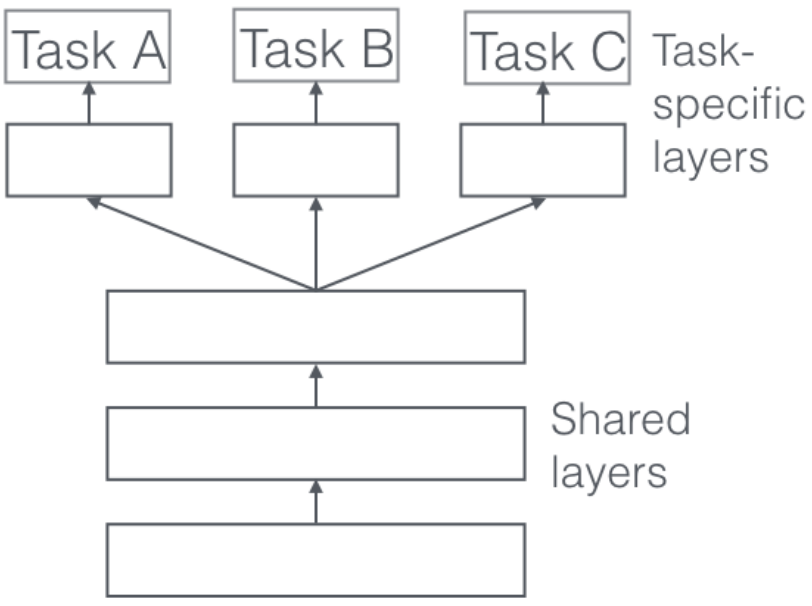
\includegraphics[scale=0.5]{figures/03_theory/03_mtl_architecture}
	\caption{Hard parameter sharing. The first three layers are shared among tasks A, B and C. Each task also has one or more layers. Source: Ruder 2017 \cite{Ruder2017}}
	\label{fig:03_mtl_architecture}
\end{figure}



\section{Transfer Learning}
\label{sec:TransferLearning}

\section{Optimization}

\subsection{Grid Search}

\subsection{Random Search}

\subsection{HyperOpt}




























\section{Methodology}
\subsection{Performance Measurements}

\subsubsection*{Precession - Recall}
The most used measure for the precision of food classifiers is the average accuracy which is calculated by dividing the number of correct matches and the total number of samples. Accuracy, however, gives no information about the underlying conditions. It is a measure of overall performance. To have a higher chance of suggesting the correct items, future systems may present a list of options that the user can chose from. Intuitively, the accuracy is much higher if a classifier can present a list of items with high confidences instead of only one item because the problem is much easier. Accuracy, however, does not measures how easy a problem is. If a classifier were able to suggest all classes as options the accuracy would always be 100\% although the results are not useful at all.

The combination of precision and recall objectively measures the actual relevance and performance of a classifier for a class of images because it includes the amount of considered items and the correct predictions. In this case the amount of considered items changes based on how many items the classifier can suggest. Precision and recall is defined as:

\begin{equation}
Precision = \frac{T_p}{T_p+F_p} \quad Recall = \frac{T_p}{T_p+F_n}.
\end{equation}

\begin{itemize}
	\item True positives $T_P$ is the number of correctly classified images of a class.
	\item False positives $F_P$ are all images that the classifier predicted to be positive but are in reality negative. {(Type I Error)}
	\item False negatives $F_N$ are all images that are positive {(belong to the class)} but are labeled as negative {(do not belong to class)} {(Type II Error)}
\end{itemize}

A high recall means that many images were matched correctly and a high precision denotes a low number of incorrectly classified images. The bigger the area under the Precision-Recall curve the better the classifier.

\subsubsection*{Null Error Rate}
The null error rate is a baseline for any classification task that calculates the accuracy if a classifier would just predict the class with the most images.

\subsubsection*{Confusion Matrix}
Confusion matrices are one of the most important metrics to understand why a classifier struggles with certain classes while getting a high precision with others. As the name suggests, a confusion matrix tells if the classifier "confuses" two classes.

A confusion matrix for $n$ classes is always a $n \times n$ matrix where columns represent the actual images classes and rows represent the predicted image classes so if the diagonal of the matrix has high values this means that the classifier makes correct predictions.

\subsubsection*{Categorical Cross-Entropy}
The categorical cross-entropy $L_i$ is an error function that is used for the training of neural networks in classification tasks as the objective function. It is more versatile than the accuracy or the \gls{mse} because it takes the deviations of the predicted label $p_{i,j}$ and the actual label $t_{i,j}$ into account and weights the "closeness" of the prediction with the logarithm. For classification, cross entropy is more useful than \gls{mse} because \gls{mse} gives too much emphasis on incorrect predictions. The categorical cross entropy function is defined as:

\begin{equation}
L_i = - \sum_{j} t_{i,j}\log(p_{i,j})
\end{equation} 

The loss values that are used for the discussion of results for neural networks are the average values of the categorical cross-entropy {(\gls{ace})}.

\subsection{Cross Validation}
Cross validation is one of the most essential techniques to evaluate real-world classification performance. Classifiers like \glspl{svm} or neural networks are always better on data they have already seen. This is called overfitting {(see section \ref{subsec:overfittingDropout})}. By training and testing on the same data the classification performance would be much better than the actual real world performance. To test if a classifier can actually work with samples it has not seen cross validation divides the dataset into different partitions. 

For most tasks it is sufficient to divide the dataset into a training and a test set. The data in the training set is used to train the classifier and the test data is used to evaluate it with data is has not seen before.

\subsubsection*{k-fold Cross Validation}
To make the classification evaluation even more robust, $k$-fold cross validation is used. By applying $k$-fold cross validation the dataset is randomly partitioned into $k$ different parts. $k-2$ parts are used for training and two parts are used for the evaluation. This process is repeated $k$-times and after each iteration the parts are exchanged so that at the end, each sample was used for training and for validation. Calculating the mean of the $k$ evaluations gives a much more robust measurement because the evaluation does not depend on the difficulty of the test partitions.

\subsection{Early Stopping}